% ===================================================================
%  Week 3 — Session 1: Convolution & Smoothing
%  Compile: pdflatex -interaction=nonstopmode -halt-on-error slides-a.tex  (twice)
% ===================================================================
\documentclass[10pt,aspectratio=169]{beamer}
% ===================================================================
%  Shared Beamer preamble for "Practical Image Processing"
%  English slides. Compile with pdfLaTeX.
% ===================================================================

\usetheme{metropolis}
\usepackage[T1]{fontenc}
\usepackage[utf8]{inputenc}
\usepackage{lmodern}
\usepackage{listings}
\usepackage{tcolorbox}
\usepackage{fontawesome5}
\usepackage{booktabs}
\usepackage{amsmath,amssymb}
\usepackage{tikz}
\usepackage{pgfplots}
\pgfplotsset{compat=1.17}
\usetikzlibrary{arrows.meta,positioning,shapes.geometric,fit,backgrounds,matrix}
\tcbuselibrary{skins,breakable}

% ---- Palette --------------------------------------------------------
\definecolor{coursePrimary}{HTML}{1B4965}   % deep blue
\definecolor{courseAccent}{HTML}{E76F51}    % coral
\definecolor{courseGood}{HTML}{2A9D8F}      % teal
\definecolor{courseBad}{HTML}{C0392B}       % red
\definecolor{courseInfo}{HTML}{2980B9}      % blue
\definecolor{codeBg}{HTML}{F5F6FA}
\definecolor{codeKw}{HTML}{8E44AD}
\definecolor{codeStr}{HTML}{2A9D8F}
\definecolor{codeCom}{HTML}{7F8C8D}

\setbeamercolor{frametitle}{bg=coursePrimary}
\setbeamercolor{progress bar}{fg=courseAccent}
\setbeamercolor{alerted text}{fg=courseAccent}
\metroset{block=fill,sectionpage=progressbar,numbering=fraction}

% ---- Code listings (Python is built into listings) -----------------
\lstdefinestyle{course}{
  backgroundcolor=\color{codeBg},
  basicstyle=\ttfamily\scriptsize,
  keywordstyle=\color{codeKw}\bfseries,
  stringstyle=\color{codeStr},
  commentstyle=\color{codeCom}\itshape,
  numberstyle=\tiny\color{codeCom},
  numbers=left, numbersep=6pt,
  showstringspaces=false, breaklines=true, breakatwhitespace=true,
  tabsize=4, columns=fullflexible,
  frame=single, framesep=4pt, rulecolor=\color{gray!30},
  keepspaces=true, upquote=true, language=Python,
}
\lstset{style=course}
\lstdefinelanguage{bash}{
  keywords={cd,pip,python,venv,source,import}, sensitive=true,
  morecomment=[l]{\#}, morestring=[b]', morestring=[b]",
}

% ---- Reusable callout boxes ----------------------------------------
\newtcolorbox{goodbox}[1][Good practice]{colback=courseGood!8,colframe=courseGood,
  fonttitle=\bfseries,title={\faCheck~#1},boxrule=0.6pt,left=4pt,right=4pt,top=3pt,bottom=3pt}
\newtcolorbox{badbox}[1][Pitfall]{colback=courseBad!8,colframe=courseBad,
  fonttitle=\bfseries,title={\faTimes~#1},boxrule=0.6pt,left=4pt,right=4pt,top=3pt,bottom=3pt}
\newtcolorbox{infobox}[1][Note]{colback=courseInfo!8,colframe=courseInfo,
  fonttitle=\bfseries,title={\faInfoCircle~#1},boxrule=0.6pt,left=4pt,right=4pt,top=3pt,bottom=3pt}
\newtcolorbox{mathbox}[1][Math]{colback=coursePrimary!6,colframe=coursePrimary,
  fonttitle=\bfseries,title={\faCalculator~#1},boxrule=0.6pt,left=4pt,right=4pt,top=3pt,bottom=3pt}

\newcommand{\keyidea}[1]{\begin{alertblock}{Key idea}#1\end{alertblock}}
\newcommand{\term}[1]{\textbf{\color{coursePrimary}#1}}
\newcommand{\code}[1]{\lstinline[basicstyle=\ttfamily\small]|#1|}

% ---- A helper to draw a small pixel grid, cells shaded by value ----
% \pixelgrid{ {10,20,120,200,240}, {30,60,130,180,230}, ... }
\newcommand{\pixelgrid}[1]{%
  \begin{tikzpicture}[font=\scriptsize,scale=0.6]
    \foreach \row [count=\ry] in {#1} {
      \foreach \val [count=\cx] in \row {
        \draw[gray,fill=coursePrimary!8] (\cx,-\ry) rectangle ++(1,-1);
        \node at (\cx+0.5,-\ry-0.5) {\val};
      }
    }
  \end{tikzpicture}}


\title{Spatial Filtering \& Convolution}
\subtitle{Week 3 — Session 1: Convolution \& Smoothing}
\author{Practical Image Processing}
\date{Lecture 3.1 \textbullet\ 60--70 min}

\begin{document}

\maketitle

\begin{frame}{Recap \& today}
  \begin{columns}[T]
    \begin{column}{0.58\textwidth}
      \begin{itemize}
        \item Wk2: point ops look at \emph{one} pixel at a time. They can brighten, threshold,
              stretch contrast — but they can't blur, sharpen, or find edges.
        \item \alert{Today (Session 1):} the \term{neighbourhood}. A small \term{kernel} slides
              over the image and combines each pixel with its neighbours. This is \term{convolution}.
        \item We build convolution from scratch, then use it for our first job: \term{smoothing}.
      \end{itemize}
    \end{column}
    \begin{column}{0.42\textwidth}
      \begin{alertblock}{Why it matters}
        Smoothing removes noise before every later stage; and convolution is the exact
        operation a CNN learns in Week 13.
      \end{alertblock}
    \end{column}
  \end{columns}
\end{frame}

\begin{frame}{Roadmap — Session 1}\tableofcontents\end{frame}

% ==================================================================
\section{From point ops to neighbourhoods}
% ==================================================================

\begin{frame}{The leap: one pixel $\rightarrow$ a window}
  \begin{columns}[T]
    \begin{column}{0.55\textwidth}
      \begin{itemize}
        \item A \term{point operation} is a function of a single value: $g(x,y)=T\big(f(x,y)\big)$.
        \item A \term{spatial filter} is a function of a whole \term{neighbourhood} around $(x,y)$.
        \item That is what lets us reason about \emph{how a pixel differs from its surroundings} —
              the basis of blur, sharpen and edges.
      \end{itemize}
    \end{column}
    \begin{column}{0.45\textwidth}
      \begin{center}
      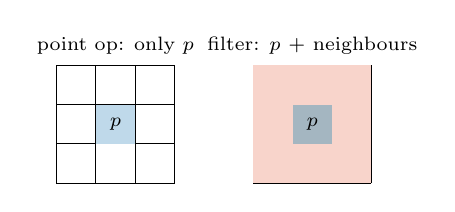
\begin{tikzpicture}[scale=0.5,font=\scriptsize]
        \foreach \x in {0,...,3} \draw (\x,0)--(\x,3);
        \foreach \y in {0,...,3} \draw (0,\y)--(3,\y);
        \fill[courseInfo!30] (1,1) rectangle (2,2);
        \node at (1.5,1.5){$p$};
        \node at (1.5,3.5){point op: only $p$};
        \begin{scope}[xshift=5cm]
        \foreach \x in {0,...,3} \draw (\x,0)--(\x,3);
        \foreach \y in {0,...,3} \draw (0,\y)--(3,\y);
        \fill[courseAccent!30] (0,0) rectangle (3,3);
        \fill[coursePrimary!40] (1,1) rectangle (2,2);
        \node at (1.5,1.5){$p$};
        \node at (1.5,3.5){filter: $p$ + neighbours};
        \end{scope}
      \end{tikzpicture}
      \end{center}
    \end{column}
  \end{columns}
  \keyidea{Point ops answer ``what is this pixel?''. Filters answer ``how does this pixel
  compare to the ones around it?''.}
\end{frame}

% ==================================================================
\section{Convolution}
% ==================================================================

\begin{frame}{A kernel slides over the image}
  \begin{center}
  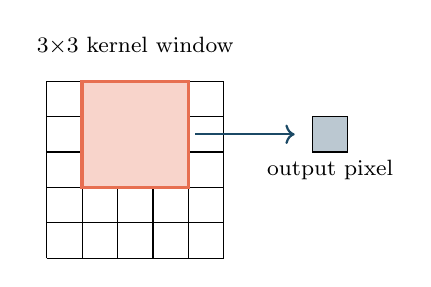
\begin{tikzpicture}[scale=0.45,font=\scriptsize]
    % image grid
    \foreach \x in {0,...,5} \draw (\x,0)--(\x,5);
    \foreach \y in {0,...,5} \draw (0,\y)--(5,\y);
    % 3x3 window highlighted
    \fill[courseAccent!30] (1,2) rectangle (4,5);
    \draw[courseAccent,very thick] (1,2) rectangle (4,5);
    \node at (2.5,6){\footnotesize 3$\times$3 kernel window};
    % output pixel
    \draw[->,coursePrimary,thick] (4.2,3.5)--(7,3.5);
    \fill[coursePrimary!30] (7.5,3) rectangle (8.5,4);
    \draw (7.5,3) rectangle (8.5,4);
    \node at (8,2.5){\footnotesize output pixel};
  \end{tikzpicture}
  \end{center}
  For each pixel: multiply the neighbourhood by the kernel, sum, write the result. Slide and repeat.
\end{frame}

\begin{frame}{Anatomy of a kernel}
  \begin{columns}[T]
    \begin{column}{0.42\textwidth}
      \begin{center}
      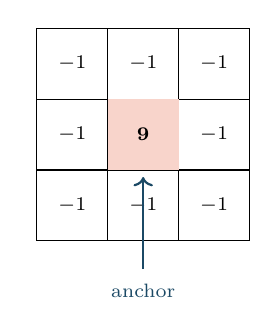
\begin{tikzpicture}[scale=0.9,font=\scriptsize]
        \foreach \x in {0,1,2,3}{\draw (\x,0)--(\x,3);}
        \foreach \y in {0,1,2,3}{\draw (0,\y)--(3,\y);}
        \fill[courseAccent!30] (1,1) rectangle (2,2);
        \node at (0.5,2.5){$-1$};\node at (1.5,2.5){$-1$};\node at (2.5,2.5){$-1$};
        \node at (0.5,1.5){$-1$};\node[coursePrimary]{}; \node at (1.5,1.5){\bfseries 9};\node at (2.5,1.5){$-1$};
        \node at (0.5,0.5){$-1$};\node at (1.5,0.5){$-1$};\node at (2.5,0.5){$-1$};
        \draw[coursePrimary,->,thick] (1.5,-0.4)--(1.5,0.9);
        \node[coursePrimary] at (1.5,-0.7){anchor};
      \end{tikzpicture}
      \end{center}
    \end{column}
    \begin{column}{0.58\textwidth}
      \begin{itemize}
        \item \term{Weights}: the numbers that multiply each neighbour.
        \item \term{Anchor} (centre): where the result is written; usually the middle of an odd-sized kernel.
        \item \term{Support / size}: how many pixels the kernel touches ($3\times3$, $5\times5$, \dots).
        \item \term{Sum} of weights: 1 for a brightness-preserving blur, 0 for an edge detector.
      \end{itemize}
    \end{column}
  \end{columns}
  \keyidea{Every filter this week is just these four choices: weights, anchor, size, sum.}
\end{frame}

\begin{frame}{Convolution, formally}
  \begin{mathbox}
    $g(x,y) = \displaystyle\sum_{i=-k}^{k}\sum_{j=-k}^{k} h(i,j)\, f(x-i,\,y-j)$
  \end{mathbox}
  \begin{itemize}
    \item $f$ = image, $h$ = kernel (a.k.a.\ filter/mask), $g$ = output; a $3\times3$ kernel has $k=1$.
    \item The kernel's values \emph{define} the operation: average $\rightarrow$ blur; differences $\rightarrow$ edges.
    \item Convolution flips the kernel (the $-i,-j$); \term{correlation} doesn't. For symmetric kernels they're identical.
  \end{itemize}
\end{frame}

\begin{frame}{Convolution vs correlation — the flip}
  \begin{columns}[T]
    \begin{column}{0.5\textwidth}
      \term{Correlation} lays the kernel down as-is:
      \[ g(x,y)=\sum_{i,j} h(i,j)\,f(x{+}i,\,y{+}j) \]
      \term{Convolution} rotates the kernel $180^\circ$ first (the $f(x{-}i,y{-}j)$).
    \end{column}
    \begin{column}{0.5\textwidth}
      \begin{itemize}
        \item For \emph{symmetric} kernels (box, Gaussian) the flip changes nothing.
        \item It matters for asymmetric kernels (gradients, Week 5).
        \item \code{cv2.filter2D} actually does \emph{correlation}; flip the kernel yourself if you need true convolution.
      \end{itemize}
    \end{column}
  \end{columns}
  \begin{infobox}
    Convolution is associative and commutative; correlation is not. That algebra is why we
    prefer convolution in theory even when the code does correlation.
  \end{infobox}
\end{frame}

\begin{frame}{Two example kernels}
  \begin{columns}[T]
    \begin{column}{0.5\textwidth}
      \term{Box blur} (average):
      \[
      \frac{1}{9}\begin{bmatrix}1&1&1\\1&1&1\\1&1&1\end{bmatrix}
      \]
      Each output = mean of its 3$\times$3 neighbourhood.
    \end{column}
    \begin{column}{0.5\textwidth}
      \term{Sharpen}:
      \[
      \begin{bmatrix}0&-1&0\\-1&5&-1\\0&-1&0\end{bmatrix}
      \]
      Boosts the centre relative to its neighbours (Session 2).
    \end{column}
  \end{columns}
  \vspace{4pt}
  \keyidea{The kernel \emph{is} the algorithm. Change the numbers, change the effect — nothing else.}
\end{frame}

\begin{frame}{Worked example: one output pixel}
  \begin{columns}[T]
    \begin{column}{0.46\textwidth}
      Image patch $P$ and box kernel $K$:
      \[ P=\begin{bmatrix}20&40&60\\80&100&120\\140&160&180\end{bmatrix} \]
      \[ K=\tfrac{1}{9}\begin{bmatrix}1&1&1\\1&1&1\\1&1&1\end{bmatrix} \]
    \end{column}
    \begin{column}{0.54\textwidth}
      \begin{mathbox}[Element-wise multiply, then sum]
        $\dfrac{1}{9}(20{+}40{+}60{+}80{+}100{+}120{+}140{+}160{+}180)$\\[2pt]
        $=\dfrac{900}{9}=\mathbf{100}$
      \end{mathbox}
      The centre becomes the \emph{mean} (100). Because the patch is a smooth ramp, the mean
      equals the centre value — a flat gradient survives a blur.
    \end{column}
  \end{columns}
\end{frame}

\begin{frame}{Edge handling: the kernel hangs off the image}
  \begin{center}
  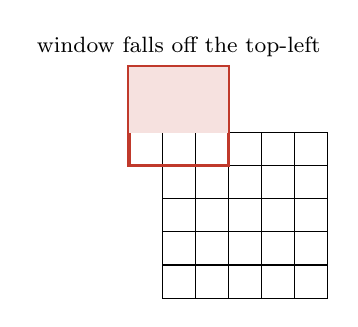
\begin{tikzpicture}[scale=0.42,font=\scriptsize]
    \foreach \x in {0,...,5} \draw (\x,0)--(\x,5);
    \foreach \y in {0,...,5} \draw (0,\y)--(5,\y);
    \draw[courseBad,very thick] (-1,4) rectangle (2,7);
    \fill[courseBad!15] (-1,5) rectangle (2,7);
    \node at (0.5,7.6){\footnotesize window falls off the top-left};
  \end{tikzpicture}
  \end{center}
  \begin{itemize}
    \item \term{Zero-pad}: treat outside as 0 — can darken borders.
    \item \term{Replicate}: repeat the edge pixel (\code{BORDER_REPLICATE}).
    \item \term{Reflect}: mirror the image across the border (\code{BORDER_REFLECT}) — usually the most natural.
  \end{itemize}
\end{frame}

\begin{frame}{Normalization: keep the brightness}
  \begin{itemize}
    \item A blur kernel should \term{sum to 1} — it preserves average brightness.
    \item An edge kernel sums to 0 — flat regions map to 0, only changes survive.
    \item Kernel not normalized $\rightarrow$ the image gets darker/brighter as a side effect.
  \end{itemize}
  \begin{badbox}
    Forgetting to normalize a blur kernel (dividing by $9$ for a $3\times3$) is why a
    ``smoothed'' image sometimes comes out too dark.
  \end{badbox}
\end{frame}

\begin{frame}[fragile]{Convolution from scratch (NumPy)}
\begin{lstlisting}[language=Python]
import numpy as np
def convolve3x3(img, k):
    k = np.flipud(np.fliplr(k))          # flip -> true convolution
    p = np.pad(img, 1, mode="reflect")   # reflect border
    out = np.zeros_like(img, dtype=float)
    for y in range(img.shape[0]):
        for x in range(img.shape[1]):
            region = p[y:y+3, x:x+3]     # 3x3 neighbourhood
            out[y, x] = (region * k).sum()
    return out
\end{lstlisting}
  This is the whole idea in nine lines. Later you replace the Python loops with \code{cv2.filter2D} for speed.
\end{frame}

\begin{frame}{Padding, numerically}
  \begin{columns}[T]
    \begin{column}{0.5\textwidth}
      Original row near the left border:
      \[ \dots\;|\;\mathbf{40}\;\;60\;\;80\;\dots \]
      \begin{itemize}
        \item \term{zero}: $\;0\;|\;40\;\;60$
        \item \term{replicate}: $\;40\;|\;40\;\;60$
        \item \term{reflect}: $\;60\;|\;40\;\;60$
      \end{itemize}
    \end{column}
    \begin{column}{0.5\textwidth}
      \begin{itemize}
        \item Zero-padding invents a dark neighbour that was never there $\rightarrow$ border darkening.
        \item Replicate/reflect reuse real data, so a blur near the edge behaves like the interior.
        \item Reflect avoids the flat ``smear'' that replicate can cause on a strong border.
      \end{itemize}
    \end{column}
  \end{columns}
  \begin{goodbox}
    Default to \code{BORDER_REFLECT} for smoothing; it keeps edge pixels honest.
  \end{goodbox}
\end{frame}

% ==================================================================
\section{Smoothing}
% ==================================================================

\begin{frame}{Box vs Gaussian blur — on a real plate}
  \begin{columns}[T]
    \begin{column}{0.33\textwidth}\begin{center}
      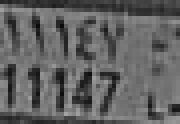
\includegraphics[width=\linewidth]{../assets/plate_gray.png}\\{\scriptsize original}
    \end{center}\end{column}
    \begin{column}{0.33\textwidth}\begin{center}
      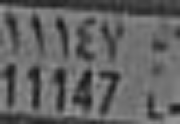
\includegraphics[width=\linewidth]{../assets/plate_box.png}\\{\scriptsize box blur 5$\times$5}
    \end{center}\end{column}
    \begin{column}{0.33\textwidth}\begin{center}
      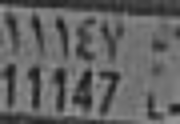
\includegraphics[width=\linewidth]{../assets/plate_gauss.png}\\{\scriptsize Gaussian $\sigma$=1.5}
    \end{center}\end{column}
  \end{columns}
  \vspace{3pt}
  Box averages equally (boxy artifacts); Gaussian weights the centre more (smoother, natural).
\end{frame}

\begin{frame}{The Gaussian kernel}
  \begin{mathbox}
    $h(i,j) = \dfrac{1}{2\pi\sigma^2}\,e^{-(i^2+j^2)/(2\sigma^2)}$
  \end{mathbox}
  \begin{itemize}
    \item \term{$\sigma$} controls the blur amount; larger $\sigma$ = more smoothing, wider kernel.
    \item \term{Separable}: a 2D Gaussian = a 1D horizontal blur then a 1D vertical blur $\rightarrow$ much faster.
    \item The go-to smoother: removes noise while preserving structure better than a box.
  \end{itemize}
\end{frame}

\begin{frame}{Building a $3\times3$ Gaussian by hand}
  \begin{columns}[T]
    \begin{column}{0.5\textwidth}
      Sample $e^{-(i^2+j^2)/2}$ at $\sigma=1$ and round to a nice integer stencil:
      \[
      \frac{1}{16}\begin{bmatrix}1&2&1\\2&4&2\\1&2&1\end{bmatrix}
      \]
      Weights fall off from the centre; they sum to $16$, so we divide by $16$.
    \end{column}
    \begin{column}{0.5\textwidth}
      \begin{itemize}
        \item Centre weight $4$ = most influence; corners $1$ = least.
        \item Sum-to-1 (after $\div16$) keeps brightness.
        \item It is the outer product of $\tfrac14[1,2,1]$ with itself — proof it is \term{separable}.
      \end{itemize}
    \end{column}
  \end{columns}
  \keyidea{A Gaussian is just a box that trusts the centre more than the corners.}
\end{frame}

\begin{frame}{Why smooth at all?}
  \begin{itemize}
    \item Remove noise before thresholding/edges (noise creates false edges — Week 5).
    \item Blur \emph{before} downsampling to avoid aliasing (Week 1's Nyquist).
    \item Suppress fine texture so large structures dominate (find the page, not the paper grain).
  \end{itemize}
  \begin{badbox}
    But blur also destroys detail. Too much and the digits smear together — a trade-off you tune.
  \end{badbox}
\end{frame}

\begin{frame}{Smoothing the water-meter image}
  \begin{columns}[T]
    \begin{column}{0.5\textwidth}\begin{center}
      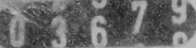
\includegraphics[width=0.9\linewidth]{../assets/meter_gray.png}\\{\scriptsize raw meter crop}\\[4pt]
      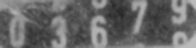
\includegraphics[width=0.9\linewidth]{../assets/meter_gauss.png}\\{\scriptsize Gaussian $\sigma$=1.5}
    \end{center}\end{column}
    \begin{column}{0.5\textwidth}
      \begin{itemize}
        \item Sensor speckle and printing texture vanish; the digit \emph{shapes} stay.
        \item This is the pre-processing step before we threshold the odometer digits in the DocScan capstone.
        \item Pick $\sigma$ big enough to kill grain, small enough to keep the strokes.
      \end{itemize}
      \begin{goodbox}
        Smooth first, then threshold. It is the single most reliable habit for clean digit masks.
      \end{goodbox}
    \end{column}
  \end{columns}
\end{frame}

\begin{frame}{Choosing the kernel size vs $\sigma$}
  \begin{itemize}
    \item Rule of thumb: kernel radius $\approx 3\sigma$, so a $\sigma=1.5$ Gaussian wants a $\approx 9\times9$ window.
    \item Too small a window \emph{clips} the Gaussian tails — you lose the smoothness you paid for.
    \item In OpenCV, pass \code{ksize=(0,0)} and let it derive the size from $\sigma$ (or vice-versa).
  \end{itemize}
  \begin{infobox}
    Odd kernel sizes ($3,5,7,\dots$) keep a well-defined centre pixel. Even sizes shift the image by half a pixel.
  \end{infobox}
\end{frame}

\begin{frame}{Blur strength on a pixel grid}
  \begin{columns}[T]
    \begin{column}{0.5\textwidth}
      \begin{center}
      A tiny image with one hot pixel:\\[3pt]
      \pixelgrid{ {20,20,20,20}, {20,20,240,20}, {20,20,20,20} }
      \end{center}
    \end{column}
    \begin{column}{0.5\textwidth}
      \begin{center}
      After a $3\times3$ box blur:\\[3pt]
      \pixelgrid{ {20,45,45,45}, {20,45,45,45}, {20,45,45,45} }
      \end{center}
    \end{column}
  \end{columns}
  \vspace{2pt}
  The single value $240$ is spread across its neighbours ($(240+8\cdot20)/9\approx45$); the
  outlier's energy is shared, so the peak drops and the surroundings rise.
\end{frame}

\begin{frame}[fragile]{Smoothing in code}
\begin{lstlisting}[language=Python]
box    = cv2.blur(img, (5, 5))              # simple average
gauss  = cv2.GaussianBlur(img, (7, 7), 1.5) # sigma = 1.5
gauss2 = cv2.GaussianBlur(img, (0, 0), 2.0) # size derived from sigma
# custom kernel via the general tool:
k = np.ones((3, 3), np.float32) / 9.0
box2   = cv2.filter2D(img, -1, k)
\end{lstlisting}
  \code{cv2.filter2D} convolves with \emph{any} kernel — the general tool you fall back to for custom filters.
\end{frame}

% ==================================================================
\section{In-class exercise}
% ==================================================================

\begin{frame}[fragile]{\faPen~In-class exercise (10 min)}
  \begin{infobox}[Blur by hand]
  \end{infobox}
  A 3$\times$3 patch with one bright speck, and the box kernel:
  \[
  P=\begin{bmatrix}10&10&10\\10&250&10\\10&10&10\end{bmatrix}\qquad
  K=\tfrac{1}{9}\begin{bmatrix}1&1&1\\1&1&1\\1&1&1\end{bmatrix}
  \]
  \begin{enumerate}
    \item Compute the box-blur output for the centre pixel.
    \item By how much did the speck's value drop? What does that tell you about box blur and noise?
    \item Would a $\tfrac{1}{16}[1,2,1;2,4,2;1,2,1]$ Gaussian give a higher or lower centre value? Why?
  \end{enumerate}
\end{frame}

\begin{frame}{\faPen~Debrief}
  \begin{itemize}
    \item Box: $(10{\cdot}8 + 250)/9 = 330/9 \approx \mathbf{37}$. The speck (250) was crushed to $\sim$37 — noise \emph{averaged away}.
    \item So a box blur is a cheap denoiser: it spreads any single bright/dark outlier across its neighbours.
    \item Gaussian: centre weight $4/16$, so $(10{\cdot}12 + 250{\cdot}4)/16 = 1120/16 = \mathbf{70}$ — \emph{higher},
          because the Gaussian trusts the centre more, so it removes less of the speck.
  \end{itemize}
  \keyidea{More centre weight $\Rightarrow$ gentler smoothing. That is the box-vs-Gaussian trade-off in one number.}
\end{frame}

% ==================================================================
\section{Wrap-up}
% ==================================================================

\begin{frame}{What you should now be able to do}
  \begin{itemize}
    \item Explain convolution and how a kernel defines an operation.
    \item Convolve a patch by hand and write a from-scratch $3\times3$ convolution.
    \item Handle borders (zero/replicate/reflect) and normalize a blur kernel.
    \item Smooth with box vs Gaussian, choose $\sigma$ and kernel size, and know the detail-vs-noise trade-off.
  \end{itemize}
\end{frame}

\begin{frame}{Next session}
  \begin{alertblock}{Session 2 — Sharpening, nonlinear \& advanced filtering}
    \begin{itemize}
      \item Sharpening: add the detail back with the \term{unsharp mask} — and the halos it causes.
      \item Nonlinear filters: \term{median} (kills salt-and-pepper) and \term{bilateral} (smooth but keep edges).
      \item The \term{low-pass / high-pass} view, \term{separability} for speed, and the bridge to CNNs.
      \item Then this week's deliverable.
    \end{itemize}
  \end{alertblock}
  \begin{center}\itshape Bring your from-scratch convolution — Session 2 builds directly on it.\end{center}
\end{frame}

\begin{frame}[standout]
  The kernel is the algorithm.\\[4pt]
  \normalsize Today: convolution, and its first job — smoothing.
\end{frame}

\end{document}
